\documentclass[11pt,          % font size: 11pt or 12pt
               ms,            % degree:    ms or phd
               onehalfspacing % spacing: onehalfspacing or doublespacing
               ]{ncsuthesis}

%%----------------------------------------------------------------------------%%
%%------------------------------ Import Packages -----------------------------%%
%%----------------------------------------------------------------------------%%

\usepackage{booktabs}  % professionally typeset tables
\usepackage{amsmath}%,amssymb,amsfonts}
\usepackage{textcomp}  % better copyright sign, among other things
\usepackage{lipsum}    % filler text
\usepackage{subfig}    % composite figures

%%%%%%%%%%%%%%%%%%%%%%%%%%%%%%%%%%%%%%%%%%
%%%%%%%%%%% Hack for alphanumeric bibliography
%%%%%%%%%%%%%%%%%%%%%%%%%%%%%%%%%%%%%%%%%%5
\RequirePackage[
			style=alphabetic,%numeric-comp,%authoryear-comp,%
			sorting=nyt,%ynt					
			hyperref=true, %	
			giveninits=true,%
			backend=bibtex,
			natbib=true,
			url=false,
			isbn=false,
			maxnames=2, %for et al to be used
			maxalphanames=1, %to avoid printing a + for every et al in abbreviation
			doi=false]{biblatex}		
			
%needed to do et al after two names
%http://tex.stackexchange.com/questions/44048/use-et-al-in-biblatex-custom-style
\renewcommand*{\finalnamedelim}{\addspace\&\space}

%Simplify abbreviation (the default uses either one or two authors and it 
%indicates et al with a +) The following five lines make it so that only the 
%first author is used in the abbreviation
%http://tex.stackexchange.com/questions/27956/label-only-from-first-author
\renewcommand*{\labelalphaothers}{}
    \renewcommand*{\intitlepunct}{}
    \DefineBibliographyStrings{german}{in={}}
    \DefineBibliographyStrings{english}{in={}}
    \DeclareNameAlias{sortname}{last-first}
    \DeclareNameAlias{default}{last-first}
	
\DeclareFieldFormat[article,periodical]{volume}{\mkbibbold{#1}}
\makeatletter

\newrobustcmd*{\parentexttrack}[1]{%
  \begingroup
  \blx@blxinit
  \blx@setsfcodes
  \blx@bibopenparen#1\blx@bibcloseparen
  \endgroup}

\AtEveryCite{%
  \let\parentext=\parentexttrack%
  \let\bibopenparen=\bibopenbracket%
  \let\bibcloseparen=\bibclosebracket}

\makeatother
\renewcommand{\cite}[1]{\parencite{#1}}

\renewbibmacro{in:}{%
  \ifentrytype{article}{}{%
  \printtext{\bibstring{in}\intitlepunct}}}
  
\AtEveryBibitem{\clearfield{month}}

\AtEveryBibitem{\clearfield{language}}

%%%%%%%%%%%%%%%%%%%%%%%%%%%%%%%%%%%%%%%%%%%%%

\addbibresource{WilliamDawn-thesis.bib}
 \defbibheading{myheading}[BIBLIOGRAPHY]{
 \chapter*{#1}
 \markboth{#1}{#1}}

%amssymb and amsfonts cannot be used in conjunction with mdput
%\usepackage{amsmath,amssymb,amsfonts}
\usepackage{dcolumn}% Align table columns on decimal point
\usepackage{bm}% bold math
%\usepackage{hyperref}% add hypertext capabilities
%\usepackage{hypernat}% make hyperref and natbib work together
\usepackage{cancel}
\usepackage{verbatim}% multiline commenting
\usepackage{ifthen}
\usepackage{url}
\usepackage{sectsty}
\usepackage{balance} 
%\usepackage{caption}
\usepackage{graphicx} %eps figures can be used instead
\usepackage{lastpage}
\usepackage[format=plain,
  justification=RaggedRight,
  singlelinecheck=false,
  font=small,labelfont=bf,
  labelsep=space]{caption} 
\usepackage{fancyhdr}
\pagestyle{fancy}

%http://tex.stackexchange.com/questions/100817/error-when-using-bc-from-abbrevs-in-caption
%Getting BC
\usepackage{abbrevs}
\usepackage{etoolbox}
\robustify{\DateMark} % after having loaded abbrevs

%Needed to solve bug from citation Hydrodynamics in 21/2 dimensions
\usepackage{units}
%see http://www.latex-community.org/viewtopic.php?f=5&t=989

\usepackage[sharp]{easylist} %used for brainstorming purposes 
% used for \Asterisk for convolution %conflicts with \widering
%\usepackage{mathabx}

%compile on single pass
%\usepackage[backend=biber,...]{biblatex}

%%%%%%%%%%%%
%%% Hack to make chapters start on odd pages
% http://tex.stackexchange.com/questions/73591/how-to-have-a-blank-even-page-before-every-chapter
%%%%%%%%%%%%
%\newcommand{\ensureoddstart}{\checkoddpage\ifoddpage\else\newpage\mbox{}\fi}
%\newcommand{\ensureoddstart}{}

%%%Fancy tables
%http://tex.stackexchange.com/questions/94032/fancy-tables-in-latex
\usepackage[table]{xcolor}
\usepackage{array,booktabs}
\usepackage{colortbl}
\newcolumntype{L}{@{}>{\kern\tabcolsep}l<{\kern\tabcolsep}}

%%%%%%%%%%
%%%%% Hack to allow more levels in outline
%%%%%%%%%%
%\setcounter{secnumdepth}{5}
%\setcounter{tocdepth}{5} %may violate ETD
%Usage http://pleasemakeanote.blogspot.com/2010/06/how-to-activate-subsubsubsection-in.html
%\section{} % level 1
%\subsection{} % level 2
%\subsubsection{} % level 3
%\paragraph{} % level 4 - equivalent to subsubsubsection
%\subparagraph{} % level 5

%http://tex.stackexchange.com/questions/60209/how-to-add-an-extra-level-of-sections-with-headings-below-subsubsection
\usepackage{titlesec}

\setcounter{secnumdepth}{4}

\titleformat{\paragraph}
{\normalfont\normalsize\bfseries}{\theparagraph}{1em}{}
\titlespacing*{\paragraph}
{0pt}{3.25ex plus 1ex minus .2ex}{1.5ex plus .2ex}

%%%%%%%%%%%%%%%%%%%%%%%%%%
%%%% Hack for containing figures within sections
%%%%%%%%%%%%%%%%%%%%%%%%%%%%
%http://ctan.org/pkg/placeins
\usepackage{placeins}
%Defines a \FloatBarrier com�mand, beyond which floats may not pass; useful,
%for example, to ensure all floats for a section appear be�fore the next 
%\section command.

%%%Hack for centering all figures
%\makeatletter
%\g@addto@macro\@floatboxreset\centering
%\makeatother

%%----------------------------------------------------------------------------%%
%%---------------------------- Formatting Options ----------------------------%%
%%----------------------------------------------------------------------------%%
%%

%% -------------------------------------------------------------------------- %%
%% Disposition format -- any titles, headings, section titles
%%  These formatting commands affect all headings, titles, headings,
%%  so sizing commands should not be used here.
%%  Formatting options to consider are
%%     +  \sffamily - sans serif fonts.  Dispositions are often typeset in
%%                    sans serif, so this is a good option. 
%%     +  \rmfamily - serif fonts
%%     +  \bfseries - bold face
%\dispositionformat{\sffamily\bfseries}   % bold and sans serif
\dispositionformat{\bfseries}            % bold and serif

%% -------------------------------------------------------------------------- %%
%% Formatting for centered headings - Abstract, Dedication, etc. headings
%%  This is where one might put a sizing command.
%%  \MakeUppercase can be used to typeset all headings in uppercase.
\headingformat{\large\MakeUppercase}   % All letters uppercase
%\headingformat{\large}                % Not all uppercase
%\headingformat{\Large\scshape}        % Small Caps, used with serif fonts.

%% Typographers recommend using a normal inter-word space after
%% sentences. TeX's default is to add an wider space, but \frenchspacing
%% gives a normal spacing. Comment out the following line if you prefer
%% wider spaces between sentences.
\frenchspacing

%% -------------------------------------------------------------------------- %%
%%  Optional packages
%%    A number of compatible packages to improve the look and feel of
%%    your document are available in the file optional.tex 
%%    (For example, hyperlinks, fancy chapter headings, and fonts)
%% To use these options, uncomment the next line and see optional.tex
%%  Optional Packages to consider.   These packages are compatible with
%%    ncsuthesis.  

%% -------------------------------------------------------------------------- %%
%% Fancy chapter headings
%%  available options: Sonny, Lenny, Glenn, Conny, Rejne, Bjarne
% \usepackage[Conny]{fncychap}
\usepackage[Rejne]{fncychap}

%%----------------------------------------------------------------------------%%
%% Hyperref package creates PDF metadata and hyperlinks in Table of Contents
%%  and citations.  Based on feedback from the NCSU thesis editor, 
%%  the links are not visually distinct from normal text (i.e. no change
%%  in color or extra boxes).
\usepackage[
  pdfauthor={William C. Dawn},
  pdftitle={SFR with FEM Multiphysics},
  pdfcreator={pdftex},
  pdfsubject={NC State ETD Thesis},
  pdfkeywords={nuclear, sodium, fast, reactor, nuclear reactor, 
    finite element, multiphysics},
  colorlinks=true,
  linkcolor=black,
  citecolor=black,
  filecolor=black,
  urlcolor=black,
]{hyperref}


%% -------------------------------------------------------------------------- %%
%% Microtype - If you use pdfTeX to compile your thesis, you can use
%%              the microtype package to access advanced typographic
%%              features.  By default, using the microtype package enables
%%              character protrusion (placing glyphs a hair past the right 
%%              margin to make a visually straighter edge)
%%              and font expansion (adjusting font width slightly to get 
%%              more favorable justification).
%%              Using microtype should decrease the number of lines
%%              ending in hyphens.
\usepackage{microtype}


%%----------------------------------------------------------------------------%%
%% Fonts 

%% ETD guidelines don't specify the font.  You can enable the fonts
%%  by uncommenting the appropriate lines.  Using the default Computer 
%%  Modern fonts is *not* required.  A few common choices are below.
%%  See http://www.tug.dk/FontCatalogue/ for more options.

%% Serif Fonts -------------------------------------------------
%%  The four serif fonts listed here (Utopia, Palatino, Kerkis,
%%  and Times) all have math support.


%% Utopia
%\usepackage[T1]{fontenc}
%\usepackage[adobe-utopia]{mathdesign}

%% Palatino
%\usepackage[T1]{fontenc}
%\usepackage[sc]{mathpazo}
%\linespread{1.05}

%% Kerkis
%\usepackage[T1]{fontenc}
%\usepackage{kmath,kerkis}

%% Times
\usepackage[T1]{fontenc}
\usepackage{mathptmx}
\usepackage{amsmath}


%% Sans serif fonts -------------------------

% this will work with math and text
%\renewcommand{\familydefault}{\sfdefault}
%\usepackage[scaled]{helvet}  % Helvetica
%\usepackage[cm]{sfmath}

%\usepackage[scaled]{berasans} % Bera Sans

%solve bug from fancyhdr in optional
%http://nw360.blogspot.com/2006/11/latex-headheight-is-too-small.html
\setlength{\headheight}{14pt}

%%----------------------------------------------------------------------------%%
%%---------------------------- Content Options -------------------------------%%
%%----------------------------------------------------------------------------%%
%% Size of committee: 3, 4, 5, or 6 -- this number includes the chair
\committeesize{4}

%% Members of committee
%%  Each of the following member commands takes an optional argument
%%   to specify their role on the committee.
%%  For co-chairs, use the commands:
%%      \cochairI{Doug Dodd}
%%      \cochairII{Chris Cox}
%%
\cochairI{Scott P. Palmtag}
\cochairII{David J. Kropaczek}
\memberI{Joseph M. Doster}
\memberII{Zhilin Li}

%% Student writing thesis, \student{First Middle}{Last}
\student{William C.}{Dawn}

%% Degree program
\program{Nuclear Engineering}

%% Thesis Title
%%  Keep in mind, according to ETD guidelines:
%%    +  Capitalize first letter of important words.
%%    +  Use inverted pyramid shape if title spans more than one line.
%%
%%  Note: To break the title onto multiple lines, use \break instead of \\.
%\thesistitle{A North Carolina State University Sample \LaTeX{} Thesis \break 
%with a Title So Long it Needs a Line Break}
\thesistitle{Sodium Cooled Fast Reactor Simulations with the Finite Element
Method}

%% Degree year.  Necessary if your degree year doesn't equal the current year.
%\degreeyear{1995}

%%----------------------------------------------------------------------------%%
%%---------------------------- Personal Macros -------------------------------%%
%%----------------------------------------------------------------------------%%

%% A central location to add your favorite macros.

%% A few examples to get you started.
\newcommand{\uv}[1]{\ensuremath{\mathbf{\hat{#1}}}}
\newcommand{\bo}{\ensuremath{\mathbf{\Omega}}}
\newcommand{\del}{\nabla}
\renewcommand{\exp}[1]{e^{#1}}
\newcommand{\Conv}{\mathop{\scalebox{1.5}{\raisebox{-0.2ex}{$\ast$}}}}%

% reference macros
\newcommand{\eref}[1]{Eq.~\ref{#1}}
\newcommand{\fref}[1]{Fig.~\ref{#1}}
\newcommand{\tref}[1]{Table~\ref{#1}}

\usepackage{color}
\newcommand{\NEW}[1]{#1}
\newcommand{\COMMENT}[1]{\textcolor{green}{#1}}

\newcommand{\NOTER}[1]{\textcolor{orange}{#1}}
\newcommand{\NOTEC}[1]{\textcolor{blue}{#1}}
\newcommand{\NOTEK}[1]{\textcolor{magenta}{#1}}

\newcommand{\mum}{\ensuremath{{\mu}\text{m}}}

%This makes it so that you can add short paths in your .tex by including the
%folders where you store your images in the search path
\graphicspath{
  {./ch01_introduction/figs/}
  {./ch02/figs/}
  {./ch03/figs/}
  {./ch04/figs/}
  }

%%---------------------------------------------------------------------------%%
\usepackage{calc}
%% Capital letter height
\newlength{\chaptercapitalheight}
\settoheight{\chaptercapitalheight}{D}
\newlength{\chapterfootskip}
\setlength{\chapterfootskip}{\chaptercapitalheight}
\addtolength{\chapterfootskip}{2\baselineskip}
% A little extra space to ensure there are 2 full double spaced lines
\addtolength{\chapterfootskip}{0.5ex}
%\def\chapterfootskipnum{\chapterfootskip}
\renewcommand{\listfigurename}{LIST OF FIGURES}
\renewcommand{\listtablename}{LIST OF TABLES}
\renewcommand{\bibname}{BIBLIOGRAPHY}

%\renewcommand{\cfttoctitlefont}{\centering\ncsu@headingformat}

%http://tex.stackexchange.com/questions/47184/height-of-figure-caption-textheight
\newlength\graphht
\newcommand\calculategraphicstargetheight[1]{%
     \setlength\graphht{\textheight 
                       -\parskip
                       -\abovecaptionskip -\belowcaptionskip
                       -(12pt * #1) % assuming baselineskip of 12pt in caption
                       -\chapterfootskip
                       }}
%\usepackage{titlesec}

%landscape support in fancyhdr from 
%http://tex.stackexchange.com/questions/9071/how-to-translate-and-rotate-the-heading-of-landscaped-pages
\usepackage{pdflscape}
\usepackage{tikz}
\fancypagestyle{lscapedplain}{%
  \fancyhf{}
  \fancyfoot{%
    \tikz[remember picture,overlay]
      \node[outer sep=1cm,above,rotate=90] at (current page.east) {\thepage};}
\renewcommand{\headrulewidth}{0pt} 
\renewcommand{\footrulewidth}{0pt}
}

\begin{document}
\pagestyle{plain}
%%---------------------------------------------------------------------------%%
\frontmatter
%% ------------------------------ Abstract ---------------------------------- %%
\begin{abstract}
  Renewed interest in advanced nuclear power reactors such as the Versatile Test 
  Reactor (VTR) at Idaho National Laboratory (INL) has encouraged enhanced 
  modeling of Sodium Cooled Fast Reactors (SFRs). Since their inception in the 
  early days of nuclear engineering with reactors such as at the Experimental 
  Breeder Reactor and Fermi 1, many new modeling techniques have been developed.
  This work seeks to introduce cutting-edge methods to the simulation of SFRs.

  In this work, the multigroup neutron diffusion equation is solved via the
  Finite Element Method (FEM). This method allows for the use of unstructured
  and general meshes. By using an unstructured mesh, physical phenomena such as
  thermal expansion can be modeled and used to perturb the mesh. Additionally,
  the FEM will allow for simplified mesh refinements by means of both geometric
  refinement and the use of higher order methods without recreating the mesh.
  The multigroup neutron diffusion equation can be solved for two-dimensional
  problems using triangles or three-dimensional problems using pentahedra, also
  known as wedges. 

  Thermal feedback effects within a SFR are also modeled in this work. A
  simplified thermal hydraulic model is used, modeling both axial heat 
  convection and radial heat conduction. Resulting temperatures are used to 
  calculate on-the-fly neutron cross-sections to capture the effects of Doppler
  feedback. Additionally, a thermal expansion model is used to simulate the 
  thermal expansion of fuel and structural components within the reactor. These 
  effects have been proven to significantly impact reactor behavior in 
  experiments such as those performed at Experimental Breeder Reactor II 
  (EBR-II).

  Using these models, a typical SFR is simulated at operating conditions. The 
  models as implemented demonstrate expected reactor behavior for an SFR and can
  be used to visualize the inherent safety features and feedback effects of such 
  a nuclear reactor.
  
\end{abstract}

%% ---------------------------- Copyright page ------------------------------ %%
\makecopyrightpage

%% -------------------------------- Title page ------------------------------ %%
\maketitlepage

%% -------------------------------- Dedication ------------------------------ %%
\begin{dedication}
  \centering To the future of clean electricity and natural beauty.
\end{dedication}

%% -------------------------------- Biography ------------------------------- %%
\begin{biography}
  William C. Dawn was born and raised in Stafford, Virginia. He attended public
  schools there for his primary education, participating in the Commonwealth
  Governor's School for High School. William earned a B.S. degree in Nuclear
  Eneingeering from North Carolina State University (NC State) in May 2017. 
  After his Master's degree, William will remain at NC State to pursue a Ph.D.
  degree in Nuclear Engineering. 

  William is a fellow of the Integrated University Program (IUP) facilitated by
  DOE-NE. During his undergraduate and graduate careers, he has had the
  opportunity to work with GE-Hitachi Nuclear Energy LLC. and Oak Ridge National
  Laboratory (ORNL). William has also made contributions to the Consortium for
  Advanced Simulation of LWRs (CASL).
\end{biography}

%% ----------------------------- Acknowledgements --------------------------- %%
\begin{acknowledgements}
  This work would not have been possible without the help of friends and family.
  I would like to thank my Mom and Dad, Suzanne and Bill Dawn, for their
  patience, their listening, and their advice. Their support has helped to make
  this work a reality.

  I would also like to thank my advisor, Dr. Scott Palmtag. We have both learned
  tremendously during this process. His consistency and desire to know more have
  kept me busy these last few months and I am grateful.
\end{acknowledgements}

%% ----------------------------- Disclaimer --------------------------- %%
\clearpage
\vspace*{\fill}
\begin{center}
  \mbox{\parbox{5in}{
  This material is based upon work supported under an Integrated
  University Program Graduate Fellowship. Any opinions, findings, conclusions,
  or recommendations expressed in this publication are those of the author and
  do not necessarily reflect the views of the Department of Energy Office of
  Nuclear Energy.
  }}
\end{center}
\vspace*{\fill}
\clearpage

\thesistableofcontents

\thesislistoftables

\thesislistoffigures

%%---------------------------------------------------------------------------%%
\mainmatter

\pagestyle{plain}
\newgeometry{margin=1in,lmargin=1.25in,footskip=\chapterfootskip, includehead, 
  includefoot}
\chapter{Introduction}
\label{ch:introduction}

\section{Motivation}
  Recent interest in advanced and next-generation nuclear power reactor designs
  has encouraged further development of modeling and simulation methods for
  these reactors. Fast reactors, a class of advanced reactors, operate with
  predominately high-energy (``fast'') neutrons in the fission reaction. Since
  early development of fast reactors, such as  \gls{ebr-i} in 1951 and Fermi 1
  in 1956, there have been significant innovations in both nuclear modeling and
  computational methods. As development of fast reactors is revisited in the
  form of the \gls{vtr} at \gls{inl}, improvements in simulation can be
  used to simulate fast reactors with modern best practices. 
  

  Nuclear reactor simulations are inherently multiphysics simulations. For
  example, neutron reaction probabilities are described by cross sections.
  Neutron cross sections are dependent on material temperatures and densities,
  both of which vary over the operating range of a nuclear power reactor. As
  reactor power changes, material temperatures and densities change, therefore
  cross sections change and affect the reactor power. The multiphysics nature
  of the reactor necessitate a simulation of the power distribution within the
  reactor as well as all feedback effects which will be modeled. 
  
  In this thesis, models for simulating fast reactors will be developed and
  demonstrated. Reactor power distribution will be modeled according to the
  multigroup neutron diffusion equation as solved by the \gls{fem} based on
  unstructured meshes with special attention to hexagonal geometries.
  The multigroup neutron diffusion solution method is verified through
  comparison to both benchmark and analytic solutions. Multiphysics effects are
  modeled including thermal hydraulics and thermal expansion. Thermal hydraulic
  effects are modeled as axial heat convection and radial heat conduction.
  Thermal expansion is modeled using simplified linear expansion models. The
  methods developed in this work can easily be used for fast reactors with a
  variety of coolants including sodium, lead, or molten salt.

  By employing a modern solution method to the neutron diffusion equation in the
  form of the \gls{fem}, the simulation can take advantage of developments in
  numerical methods including the solution of linear systems. Additionally, the
  simulation allows for the incorporation of generalized multiphysics effects
  whereas current state-of-the-art techniques (such as \dif) require data
  processing and manual iteration to simulate multiphysics effects. Ultimately, 
  the simulation is designed to simulate an operating fast reactor and estimate
  feedback coefficients by coupling multiphysics models.

\section{Geometry Description}
  \label{sec:geometry_description}
  The high-energy neutron spectra inherent to fast reactors results in
  relatively small neutron cross sections compared to larger cross sections in
  the thermal energy range. To compensate for this fact, fast reactors are
  typically designed with hexagonal, triangularly pitched, fuel assemblies to
  maximize fuel packing. An example of a fast reactor with hexagonal fuel
  assemblies is shown in \fref{fig:reactor_materials}.
  
  \begin{figure}
    \centering
    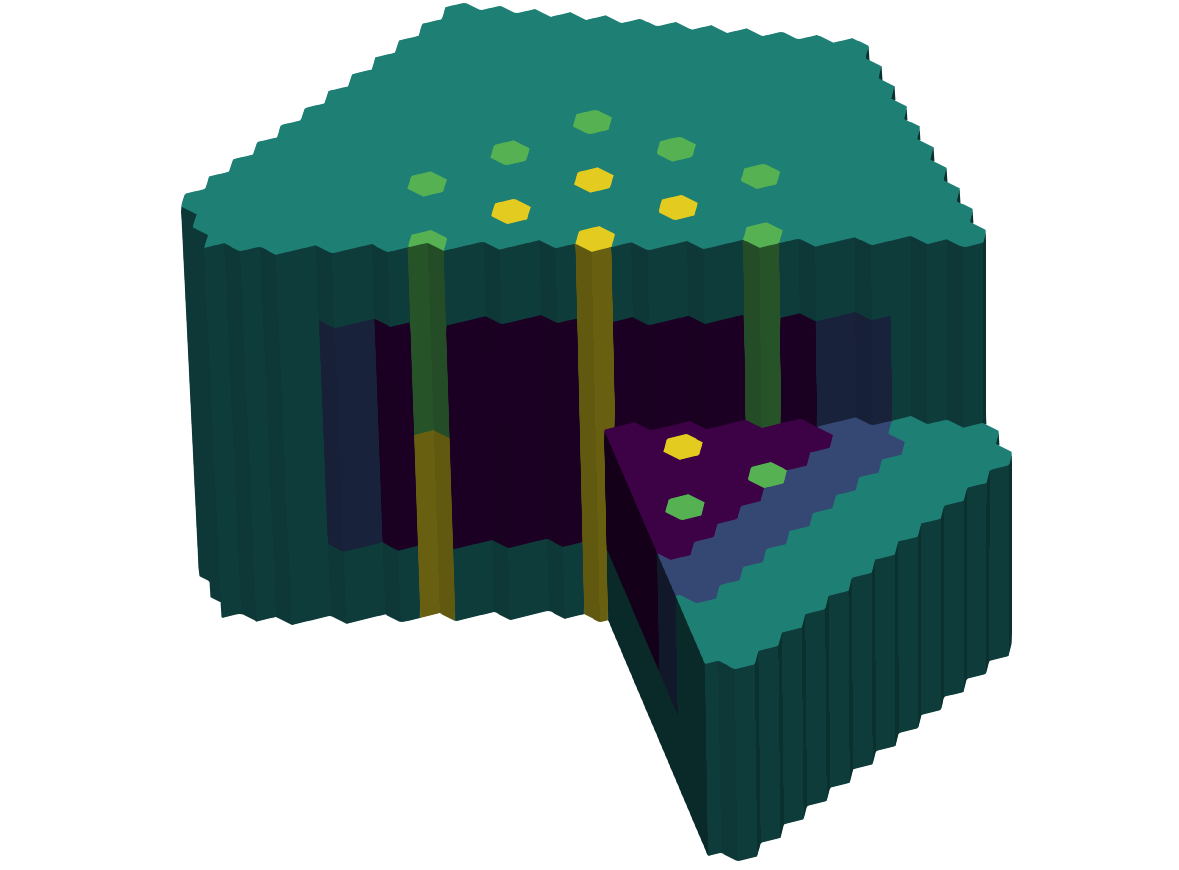
\includegraphics[width=\textwidth]{reactor_materials}
    \caption{Example of Fast Reactor Materials based on MONJU.}
    \label{fig:reactor_materials}
  \end{figure}

  \begin{figure}
    \centering
    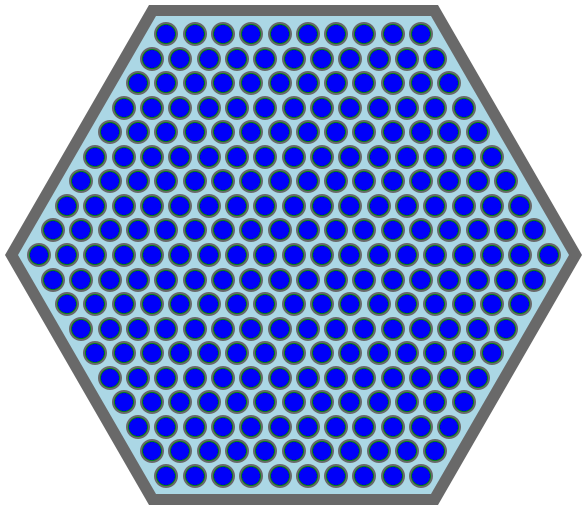
\includegraphics[width=0.5\textwidth]{prism_hex}
    \caption{Example of Fast Reactor Fuel Assembly Cross Section.}
    \label{fig:prism_hex}
  \end{figure}

  A cross-sectional representation of a hexagonal fuel assembly is shown in
  \fref{fig:prism_hex}. This geometry is used in the homogenization of neutron
  cross sections and is also used to describe coolant flow geometries.
  Dimensions of assemblies are measured at room temperature and will later be
  expanded according to the thermal expansion model in
  \chref{ch:thermalExpansion}.

  Note the individual rods in \fref{fig:prism_hex} are cylindrical and are
  arranged into a hexagonal assembly. The basic geometry is a metallic fuel
  material within stainless steel cladding. The gap between the fuel and
  cladding is filled by sodium bond to improve thermal conductivity across the
  gap. The rod is helically wrapped by a steel wire to ensure separation between
  rods that will allow for coolant flow. The wire wrap also serves to encourage
  the mixture of coolant within the assembly. (Note: wire wrap is omitted from
  \fref{fig:prism_hex}.) Many rods are then assembled into an assembly and
  surrounded by a hexagonal can made of steel. This can aids in structural
  stability and prohibits cross-flow of coolant between assemblies. 

  The dimensions within a single rod are shown in \fref{fig:pin_model} and the
  dimensions within a hexagonal assembly can are shown in \fref{fig:hex_can}. In
  \fref{fig:hex_can}, $T\!h_{can}$ is the thickness of the assembly can,
  $F\!2\!F$ is the flat-to-flat measurement of the outside of the hexagonal can,
  and \textit{Pitch} is the distance between the center of two rods. Using the
  geometry described in these figures, the material cross-sectional areas are
  calculated according to the given formulae where $N_{rod}$ is the number of
  rods in the assembly and $A\!P$ is the assembly pitch. $A\!P > F\!2\!F$ to
  account for inter-assembly sodium gaps (see ``Gap'' in \fref{fig:hex_can}).
  \begin{align}
    \label{eq:afrac_first}
    A_{total} &= \frac{\sqrt{3}}{2} A\!P^2 \\
    A_{box} &= 
      \frac{\sqrt{3}}{2} \left(F\!2\!F^2 - \left(F\!2\!F - 2
      Th_{can}\right)^2\right) \\
    A_{wrap} &= N_{rod} \frac{\pi}{4} D_{wrap}^2 \\
    A_{clad} &= N_{rod} \pi (R_C^2 - R_B^2) \\
    A_{bond} &= N_{rod} \pi (R_B^2 - R_F^2) \\
    A_{fuel} &= N_{rod} \pi R_F^2 \\
    A_{cool} &= A_{total} - A_{box} - A_{wrap} - A_{clad} - A_{bond} -
      A_{fuel}\\
    \label{eq:afrac_last}
    A_{struct} &= A_{box} + A_{wrap} + A_{clad}
  \end{align}
  Calculating the areas as above allows for calculation of cross-sectional area
  fractions. Assuming constant dimensions in the axial direction, these area
  fractions are equivalent to volume fractions and are useful for neutron
  cross section homogenization. Additionally, these formulae allow for thermal
  expansion as the liquid sodium in the bond and the liquid coolant are allowed
  to vary to allow for the expansion of other materials.

  \begin{figure}
    \centering
    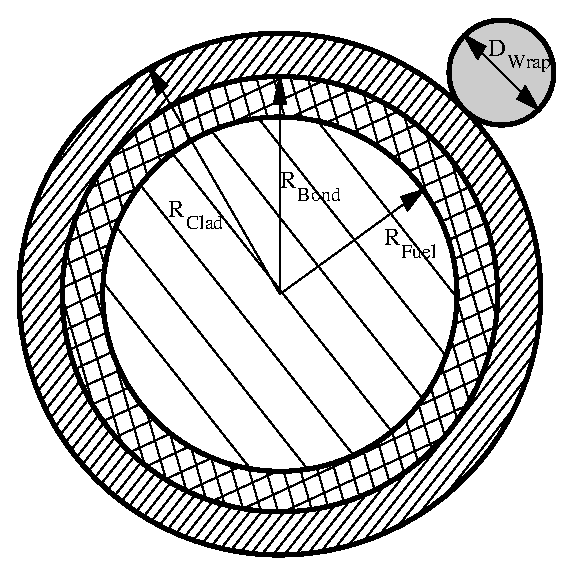
\includegraphics[width=0.6\textwidth]{pin_model}
    \caption{Dimensions of Thermal Hydraulic Rod Model (not to scale).}
    \label{fig:pin_model}
  \end{figure}

  \begin{figure}
    \centering
    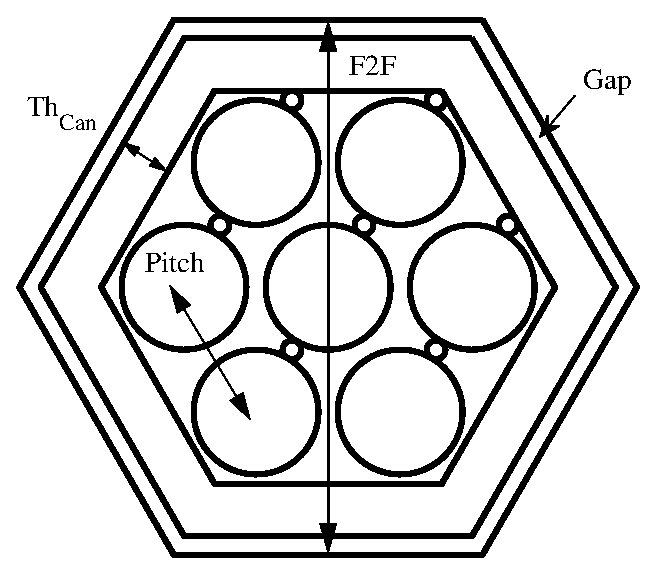
\includegraphics[width=0.6\textwidth]{hex_can}
    \caption{Dimensions of Hexagonal Can (not to scale).}
    \label{fig:hex_can}
  \end{figure}

\section{Cross Section Treatment}
  \label{sec:cross_section_treatment}
  Reactor materials are ``smeared'' into homogeneous regions. This treatment is
  common to fast reactors because of the relatively large neutron
  mean-free-paths compared to the scale of material dimensions. Additionally,
  the neutron distribution will be modeled using the neutron diffusion equation
  which cannot accurately resolve small geometric details. The natural
  choice for these homogeneous regions are the hexagonal assemblies themselves.
  Materials are permitted to be heterogeneous axially. For this work, four
  distinct regions are modeled within a hexagonal assembly: fuel, bond, coolant,
  and steel. Steel material includes cladding, wire wrap, and assembly can. 
  These four regions are then homogenized into a hexagonal assembly.

  For simplified analytic and benchmark problems, cross sections are specified
  by the problem. For realistic simulations, multigroup microscopic cross
  sections are generated using the computer program \mcc \cite{mcc}. The cross
  section generator uses 2,082 fine energy groups to collapse down to an
  arbitrary number of coarse energy groups. For this simulation, the recommended
  and default 33-group energy structure is used. However, the methods in this
  work are implemented generally and are not dependent on a particular energy
  group structure. \mcc solves the infinite-homogeneous (zero-dimension) neutron
  transport equation for isotopic number densities as input by the user.  Cross
  sections for each assembly type are generated separately to accurately
  simulate the neutron energy spectrum within the assembly. This procedure
  results in a unique material cross sections for each assembly type. For
  example, each assembly type contains steel; therefore, there will be a
  separate steel cross section for each assembly type in the cross section
  library. Within \mcc, the neutron energy spectrum for fissile media is
  generated by the media's fission spectrum.  Non-fissile homogenized mixtures,
  such as control assemblies or reflector assemblies, the default
  \isotope[238]{U} fission spectrum is assumed.

  Cross section libraries are generated for several different temperatures to
  capture temperature-dependent cross section effects. These libraries are then
  used during the simulation to calculate cross sections as a function of
  material temperatures. The fuel, clad, and coolant temperatures in a
  simulated reactor can be calculated with a thermal hydraulic model (see
  \chref{ch:thermalHydraulics}). However, the temperatures calculated in the
  thermal hydraulic model are functions of reactor power and coolant mass flow
  rate. These parameters are not known before the simulation for a general
  reactor. Instead, a simplified one-dimensional, single-channel model is used
  to estimate temperatures for cross section library generation. This model is
  based on the axial convection and radial conduction models in
  \chref{ch:thermalHydraulics}. The simulation model can use general cross
  section library temperatures and a general number of temperature libraries.
  A user may select the number of cross section libraries and specify the
  temperatures for which the libraries apply in a general manner. Typical 
  cross section library temperatures for simulating liquid metal cooled, metal
  fueled, fast reactors are given in \tref{tab:xstemps}.

  \begin{table}
    \caption{Temperatures Selected for Cross Section Libraries.}
    \label{tab:xstemps}
    \begin{center}
      \begin{tabular}{crrr}
        \toprule
        Library & $T_{cool} \units{K}$ & $T_{clad} \units{K}$ & 
          $T_{fuel} \units{K}$ \\
        \midrule
        1 & 628.15 & 628.15 & 628.15  \\
        2 & 708.65 & 757.50 & 807.15  \\
        3 & 896.87 & 920.47 & 961.46 \\
        4 & 1072.81 & 1114.83 & 1183.14 \\
        \bottomrule
      \end{tabular}
    \end{center}
  \end{table}

  Note that the maximum temperatures in \tref{tab:xstemps} are greater than 
  temperatures observed at typical reactor operating conditions. This is
  necessary so that even at perturbed reactor conditions (e.g. $110\%$ full
  power), the peak core temperatures can still be interpolated within the
  libraries.

  Cross sections are homogenized within each hexagonal assembly using isotopic
  microscopic cross sections from \mcc and user input number densities.
  Homogenization is performed in two steps: first, isotopic homogenization and
  second, volumetric homogenization. Isotopic homogenization is performed by
  summing microscopic cross sections and associated number densities. Let
  $\sigma_{i,j,x,g}$ represent the microscopic cross section for isotope $i$, in
  region $j$, for reaction type $x$, and energy group $g$ as output by \mcc.
  $\sigma_{i,j,x,g}$ has units of area. Then, let $N_{i,j}$ represent the atom
  number density for isotope $i$ in region $j$ as input by the user. $N_{i,j}$
  has units of inverse volume. The macroscopic cross section can then be
  defined
  \begin{equation}
    \label{eq:isotopic_homogenization}
    \Sigma_{j,x,g} = \sum_{i=1}^{N_{iso}} N_{i,j} \, \sigma_{i,j,x,g}
  \end{equation}
  where $\Sigma_{j,x,g}$ is the macroscopic cross section in region $j$, for
  reaction type $x$, and energy group $g$. In \eref{eq:isotopic_homogenization},
  $N_{iso}$ represents the number of isotopes in region $j$. Note that
  $\Sigma_{j,x,g}$ will have units of inverse length.

  Next, volumetric cross section homogenization is performed using volume
  fractions. Assuming dimensions do not change axially within a hexagonal
  assembly, the areas calculated in \eref{eq:afrac_first} through
  \eref{eq:afrac_last} can be used to calculate area fractions.
  These area fractions can subsequently be treated as volume fractions.
  Using the definition of macroscopic cross sections from
  \eref{eq:isotopic_homogenization}, the volumetrically homogenized macroscopic
  cross section is 
  \begin{equation}
    \label{eq:volumetric_homogenization}
    \Sigma_{x,g} = \frac{\sum_{j = 1}^{N_{reg}} \Sigma_{j,x,g} \, V_j}
      {\sum_{j=1}^{N_{reg}} V_j}
  \end{equation}
  where $V_j$ is the volume or area occupied by region $j$ in the hexagonal
  assembly and $N_{reg}$ is the number of regions in the hexagonal assembly.
  Typically, $N_{reg} = 4$ with unique regions for fuel, sodium bond, sodium
  coolant, and steel structural material. After homogenizing cross sections
  isotopically and volumetrically, the diffusion coefficient for energy group
  $g$, $D_g$, can be calculated as 
  \begin{equation}
    \label{eq:diffusion_homogenization}
    D_g = \frac{1}{3 \Sigma_{tr,g}}
  \end{equation}
  where $\Sigma_{tr,g}$ represents the macroscopic transport cross section for
  energy group $g$. $\Sigma_{tr,g}$ has been homogenized according to
  \eref{eq:isotopic_homogenization} and \eref{eq:volumetric_homogenization}.
  Note that $D_g$ will have units of length.

\section{Thesis Organization}
  In \chref{ch:neutronDiffusion}, the derivation of the \gls{fem} solution to
  the multigroup neutron diffusion equation is presented. Special attention is
  paid to triangular and wedge elements. The resulting eigenvalue problem is
  solved using the Power Method. Results from the diffusion solution are
  verified in two-dimensional and three-dimensional problems with both analytic 
  and benchmark solutions. These verification problems for the neutron diffusion
  equation are presented in \chref{ch:diffusionResults}.

  \chref{ch:thermalHydraulics} presents the formulation of axial heat convection
  and radial heat conduction models for a typical fast reactor. These models are 
  used to calculate material temperatures and update cross sections for the 
  simulation. Results of the numerical model are compared to analytical models 
  and example material temperatures are shown.

  In \chref{ch:thermalExpansion} a simplified thermal expansion model is
  presented. The model assumes linear thermal expansion for given material
  properties and user-specified thermal expansion temperatures. A simple
  demonstration of the effects of thermal expansion on reactivity are presented.

  The combination of all of these models allows for the realistic simulation of
  a fast reactor. In \chref{ch:coupledResults}, the multiphysics models are
  coupled and investigated for a benchmark reactor problem. Using this benchmark
  reactor and the models described, multiphysics reactivity feedback
  coefficients are estimated.
 
  Finally, \chref{ch:conclusions} presents a summary and the conclusions of this
  research. Additionally, recommendations for further research are provided.

\chapter{INTRODUCTION}
\label{chap-one}
Let's start with a few paragraph basics, here is how to make \textbf{bold}, 
and \textit{italics}, and \emph{emphasized}.  Let's say you need to cite 
something in your references, simply type \verb^\cite{key}^, which produces
\cite{einstein1935particle}.  
Some other references are \cite{golub1996matrix} and 
\cite{larsen1974asymptotic}.
Some \LaTeX{} compilers 
require a second compilation for citations and references 
to be sorted and matched properly in the resulting document.  

Here is a quotation:
\begin{quotation}
Alice, Bob and Carol are boring.  Who would even want to know their secret?
\end{quotation}

Let's say we need to make a list, try this on for size
\begin{enumerate}
  \item NCSU is great
  \item I like NCSU
  \item I really hope I can find a job when I graduate!
\end{enumerate} 

\section{Math enviroments}
\subsection{Equations}

There are many different ways to write equations, for example we could put 
$a^2 + b^2 = c^2$ directly into a sentence.  Or we could use the equation 
enviroment and do 
%
\begin{equation}
  a^2+b^2=c^2.
  \label{eq:one}
\end{equation} 
And from here we can later reference it by simply doing typing 
\verb^\ref{label}^, which gives \ref{eq:one}.  However, defining and using
equation and figure reference macros will ensure that the equation
references are consistent, instead of having Eq.~(1), Equation 3, Eqn 4
scattered through the thesis.  This template file defines \verb^\eref^
and \verb^\fref^ for this purpose. You can modify the macros to your liking
in the \texttt{YourName-thesis.tex} file.
For example, the command \verb^\eref{label}^ gives \eref{eq:one}.


If you don't need to reference an equation you may simply do this 
\[
  a^2 + b^2 = c^2.
\]

For Greek letters you must go to the math enviroments, for example 
$\alpha$, $\beta$, and $\gamma$.  Let's look at equations that cover 
multiple lines, none of these equations may be true or mean anything, but so 
that the reader can get some ideas.  In addition I will use some other useful 
notations like subscripts, superscripts, fractions, etc.  One important item 
of note is that one uses the ``ampersand" symbol to line up equations 
(also look at how I used quotations).
%
\begin{eqnarray}
\gamma_1 & = & \alpha^{\beta} + \psi_0 \frac{\psi_1}{\psi_2+\psi_3} \label{eq.two} \\
& = & \beta_1 + \beta_2 + \ldots + \beta_k \nonumber\\
& \rightarrow & E(\gamma_2) 
\end{eqnarray}

Alternatively, one can specify a slightly different enviroment if none of 
the equations need to be numbered.  Remember that if you are planning on 
referring to them later on, you must use a ``label" statement.
%
\begin{eqnarray*}
\gamma_1 & = & n^{-1/2} \displaystyle \sum_{i=1}^n \left[h(X_i,\beta_0)-E\{h(X_i,\beta_0)\}\right]\\
& \rightarrow & \hat q \pm \frac{\partial \gamma_2}{\partial \beta}. 
\end{eqnarray*}  
Lastly there may be times in which you want to use a non-italicized word 
your formula, such as an indicator function that may look like this 
$\mbox{I}\{\mu_i(1,\beta)>\mu_i(0,\beta)\}$ , if so just use the 
``mbox" statement.


You could use a multiline equation for long equations.  The environment
is \texttt{multline}.  Insert \verb^\\^ for line breaks.

\begin{multline*}
\bo \cdot \vec{\nabla} \psi(\vec{r},\bo ,E) + \Sigma_t(\vec{r},E)\psi(\vec{r},\bo ,E) = \\
  \int_{4\pi} d\bo' \int_0^{\infty} dE' \, \Sigma_s(\vec{r},\bo'\to\bo,E'\to E)\psi(\vec{r},\bo',E') + Q(\vec{r},\bo ,E),
\end{multline*}


we operate with $\displaystyle\int_{0}^{\infty}\left(\,\cdot\,\right) dE$
to obtain
\begin{multline*}
  \bo \cdot \vec{\nabla} \tilde{\psi}(\vec{r},\bo)
  + \Sigma_t(\vec{r})\tilde{\psi}(\vec{r},\bo) = \\
  \int_{4\pi} d\bo' \int_0^{\infty} dE' \, \psi(\vec{r},\bo',E')
  \left [ \int_{0}^{\infty} dE \, \Sigma_s(\vec{r},\bo'\to\bo,E'\to E)
  \right ] + \tilde{Q}(\vec{r},\bo),
\end{multline*}


\chapter{TABLES, FIGURES AND MATRICES}
\label{chap-two}
In Chapter \ref{chap-one} we did some typesetting and equations; now let's 
look at tables, figures, and matrices.

\section{Tables}
Table \ref{tab:one} is about as simple as they come, to put a formula in a 
table just use the same methods as putting a formula in a paragraph.  
Table \ref{tab:two} is a similar table in landscape on a seperate page.  
%
\begin{table}
\caption{Table Example}
\label{tab:one}
\begin{center}
\begin{tabular}{lccl}
\toprule
Treatment & No Death & Death & Total\\
\midrule
Therapy A & 1295 & 72 & 1367\\
Therapy B 	& 2294 & 195 & 2489\\
\midrule
Total & 3589 & 267 & 3856\\
\bottomrule
\end{tabular}
\end{center}
\end{table}

\paragraph{Filler Text} \lipsum[1-2]

\newgeometry{margin=1in,lmargin=1.25in,footskip=\chapterfootskip, includehead, includefoot}
\thispagestyle{lscapedplain}
\begin{landscape}
\begin{table}
\caption{Landscape Table Example}
\label{tab:two}
\begin{center}
\begin{tabular}{lcccccccccl}
\toprule
Patient & A & B & C & D & E & F & G & H &I & Total \\
\midrule
John & 1 & 2 & 3 & 4 & 5 & 6 & 7 & 8 & 9 & 45 \\
Amy & 1 & 2 & 3 & 4 & 5 & 6 & 7 & 8 & 9 & 45 \\
Jim & 1 & 2 & 3 & 4 & 5 & 6 & 7 & 8 & 9 & 45 \\
Jason & 1 & 2 & 3 & 4 & 5 & 6 & 7 & 8 & 9 & 45 \\
Sandy & 1 & 2 & 3 & 4 & 5 & 6 & 7 & 8 & 9 & 45 \\
Icem & 1 & 2 & 3 & 4 & 5 & 6 & 7 & 8 & 9 & 45 \\
\midrule
Total & 6 & 12 & 18 & 24 & 30 & 36 & 42 & 48 & 54 & 270\\
\bottomrule
\end{tabular}
\end{center}
\end{table}
\end{landscape}
\restoregeometry
\pagestyle{plain}
\thispagestyle{plain}
\newgeometry{margin=1in,lmargin=1.25in,footskip=\chapterfootskip, includehead, includefoot}


\section{Figures}

The easiest way to insert a picture is to have that picture in pdf format.  
\fref{fig:hist1} and \fref{fig:hist2} are two figures typeset normally.
ETD guidelines allow the use of landscape pages in the electronic 
submission.  To rotate a page, do NOT use the \texttt{lscape} environment. 
Instead, use the \texttt{pdflscape} package, for compatibility with PDFlatex.
Please note, if you are preparing a document for binding, consider
giving the \texttt{hardcopy} option in the \verb|\documentclass|
declaration.  This will place the page number at the normal location,
which is where it should be for printing and binding.

\begin{figure}[hbtp]
\centering
  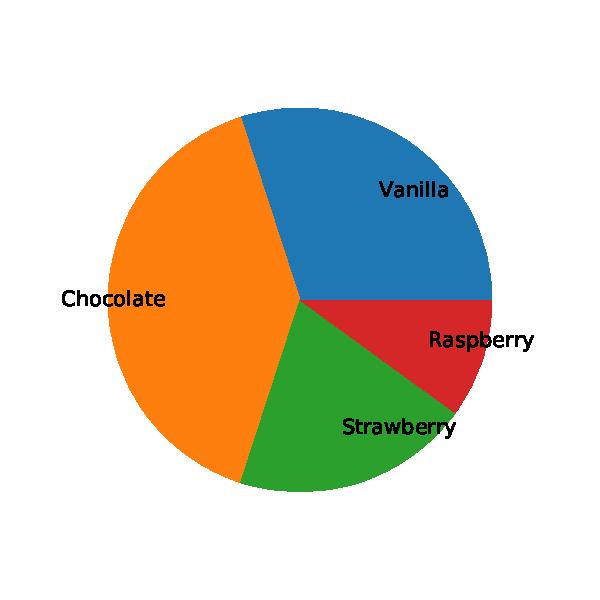
\includegraphics[width=0.6\textwidth]{pie}%{Chapter-2/figs/pie}
\caption{Here is a sample figure}
\label{fig:hist1}
\end{figure}

For an example of a figure with a really long caption, see Fig.~\ref{fig:longcap}
\begin{figure}[hbtp]
\centering
\calculategraphicstargetheight{11}
  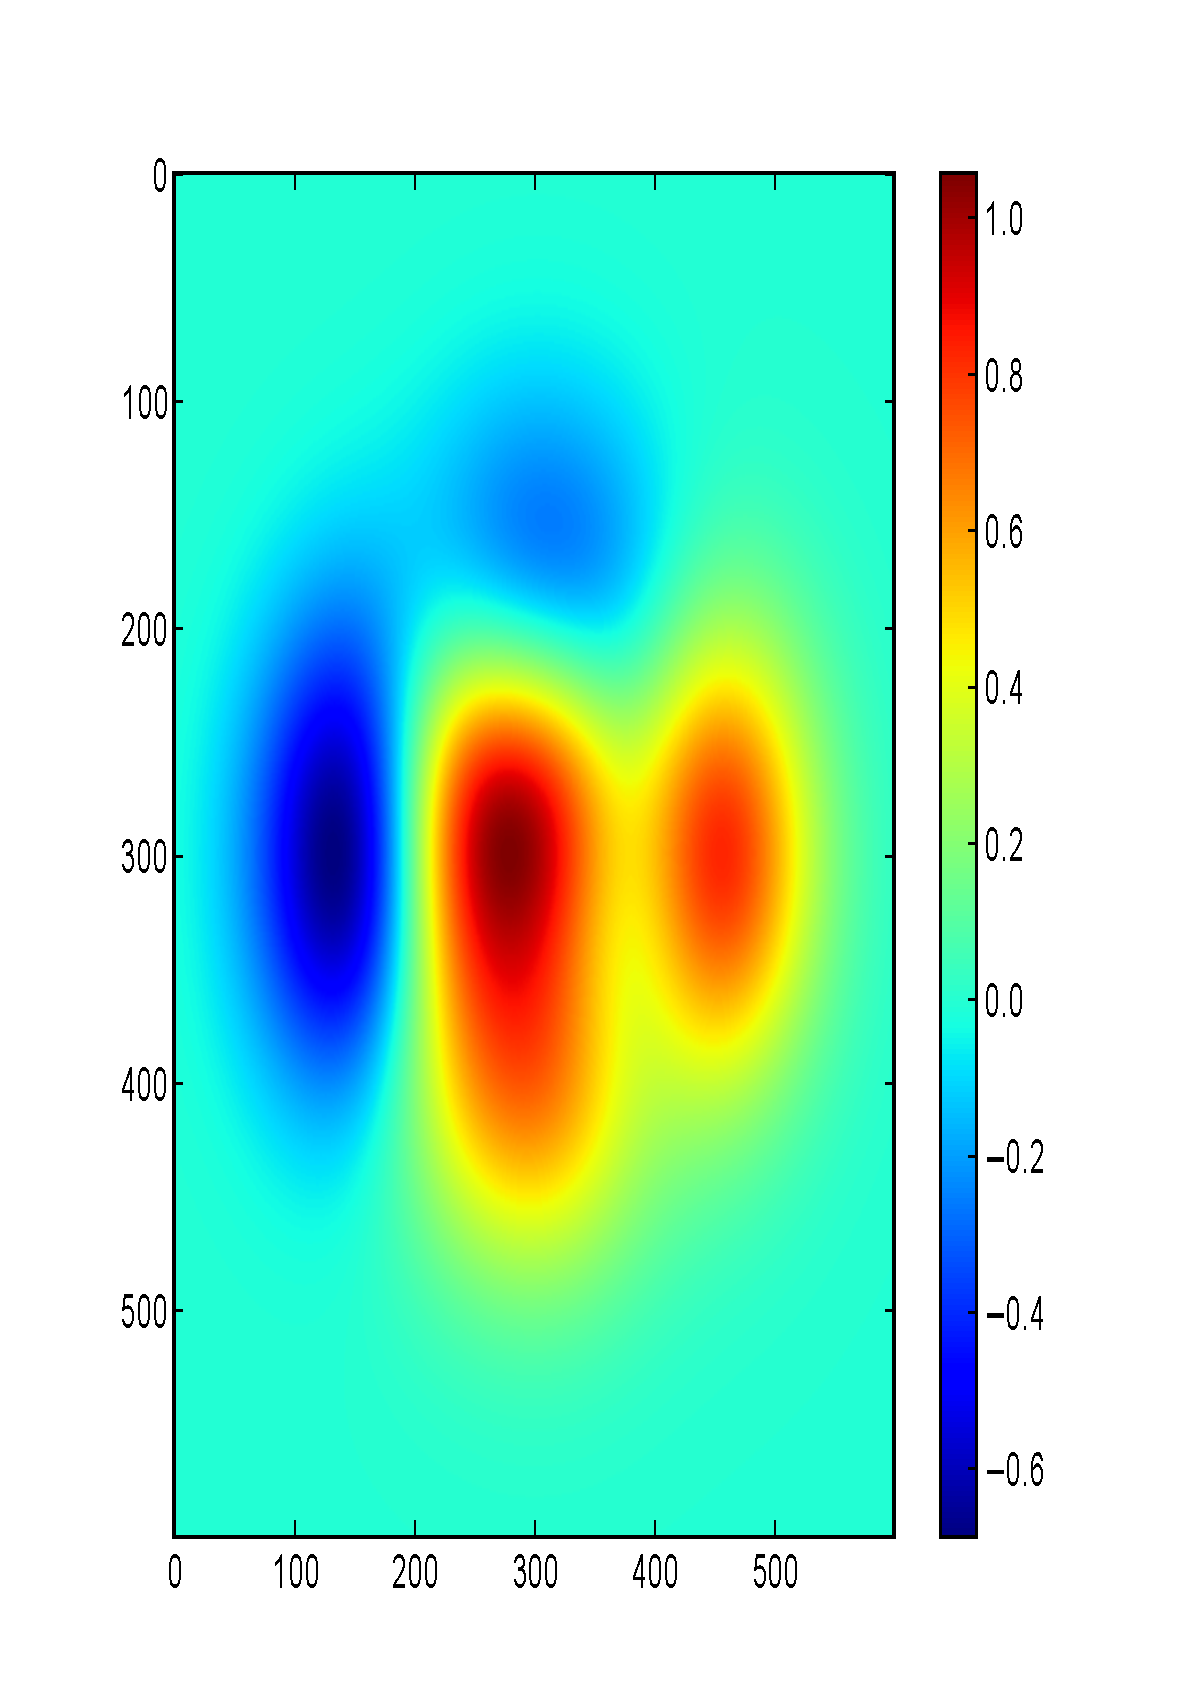
\includegraphics[height=\graphht]{color_stretched}%{Chapter-2/figs/color_stretched}
\caption{Here is a HUGE sample figure with a HUGE caption. Our goal is to make 
  a caption that is so long that the caption spills into the lower margin, 
  leading to an ETD error. The way to solve this problem in a systematic way is
  to calculate how many lines of text the caption will use, then adjust the size
  of the image, such that it leaves just enough space for your huge caption.
  How I am solving this problem is by providing a new variable called graphht 
  that stores how tall the image should be. Then, to calculate how tall to make 
  the figure, you use the new function that I am providing called
  calculategraphicstargetheight. This function has one argument. The argument
  of the function is how many lines of text you estimate that the caption
  occupies. You can always run your tex once, measure this number, and type it
  into the argument for the function. What the function will do (it is defined 
  in the preamble) is take into account the size you give it, the spacing of the
  chapter and the footer at the bottom, and then calculate the total vertical 
  space available. Thus, this function should be used for images that are taller
  than they are wide.}
\label{fig:longcap}
\end{figure}
%
\begin{figure}[hbtp]
\centering
  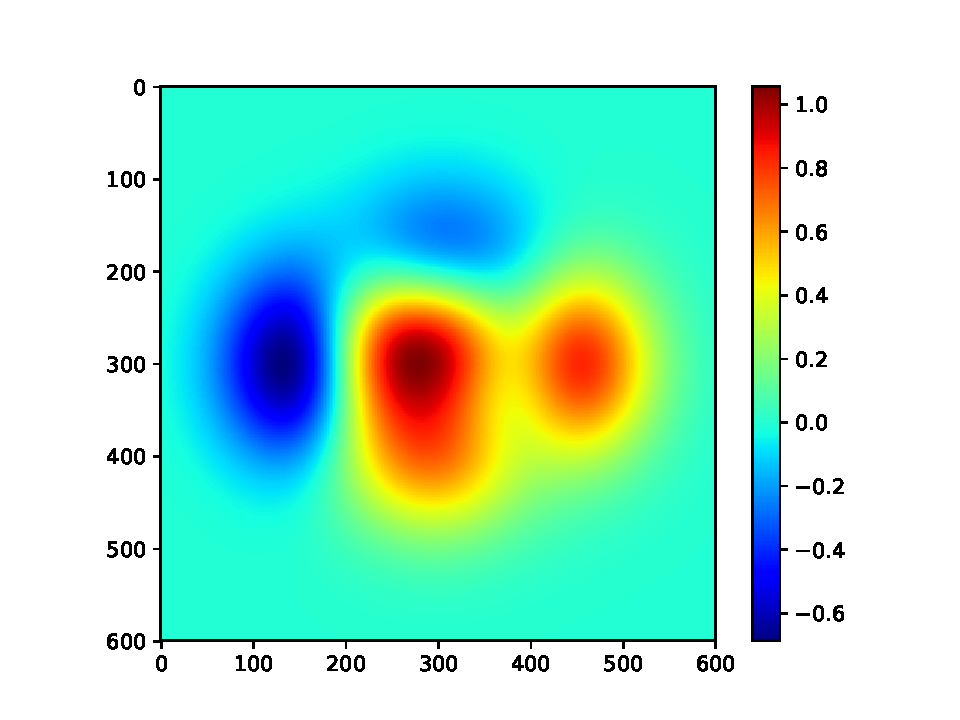
\includegraphics[width=0.6\textwidth]{color}%{Chapter-2/figs/color}
\caption{Here is a sample figure}
\label{fig:hist2}
\end{figure}
%
\begin{figure}[hbtp]
\centering
\subfloat[]{
  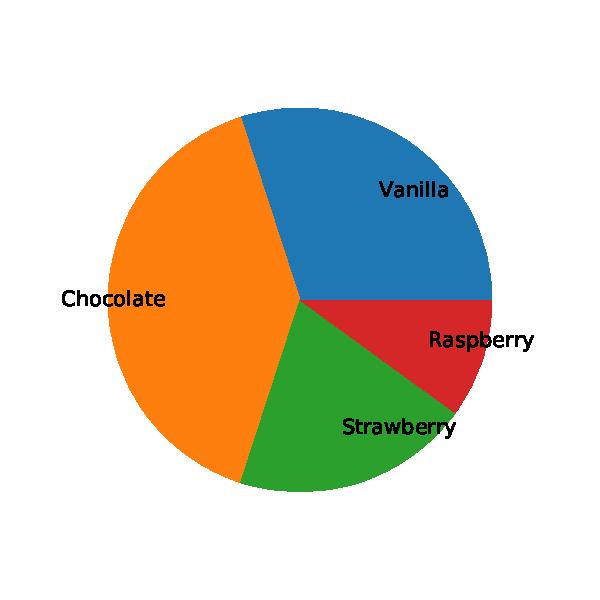
\includegraphics[width=0.4\textwidth]{pie}%{Chapter-2/figs/pie}
}
\subfloat[]{
  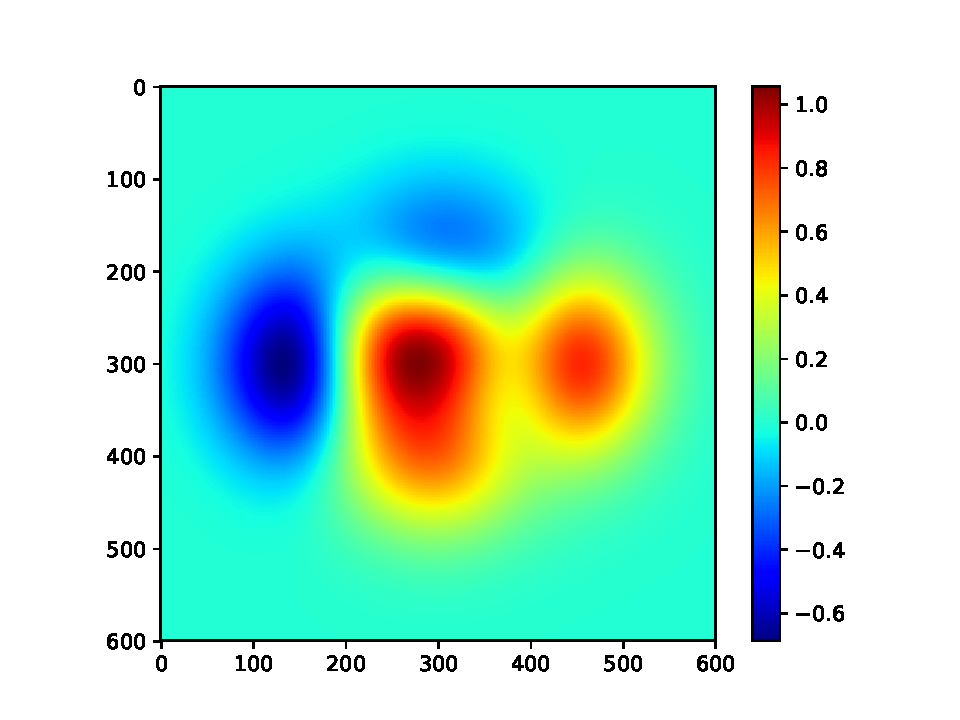
\includegraphics[width=0.4\textwidth]{color}%{Chapter-2/figs/color}
}
\caption{Here are two floating subfigures}
\label{fig:subfigures}
\end{figure}


\paragraph{Filler Text} \lipsum[12-15]

\newgeometry{margin=1in,lmargin=1.25in,footskip=\chapterfootskip, includehead, includefoot}
\thispagestyle{lscapedplain}
\begin{landscape}
\begin{figure}
\centering
  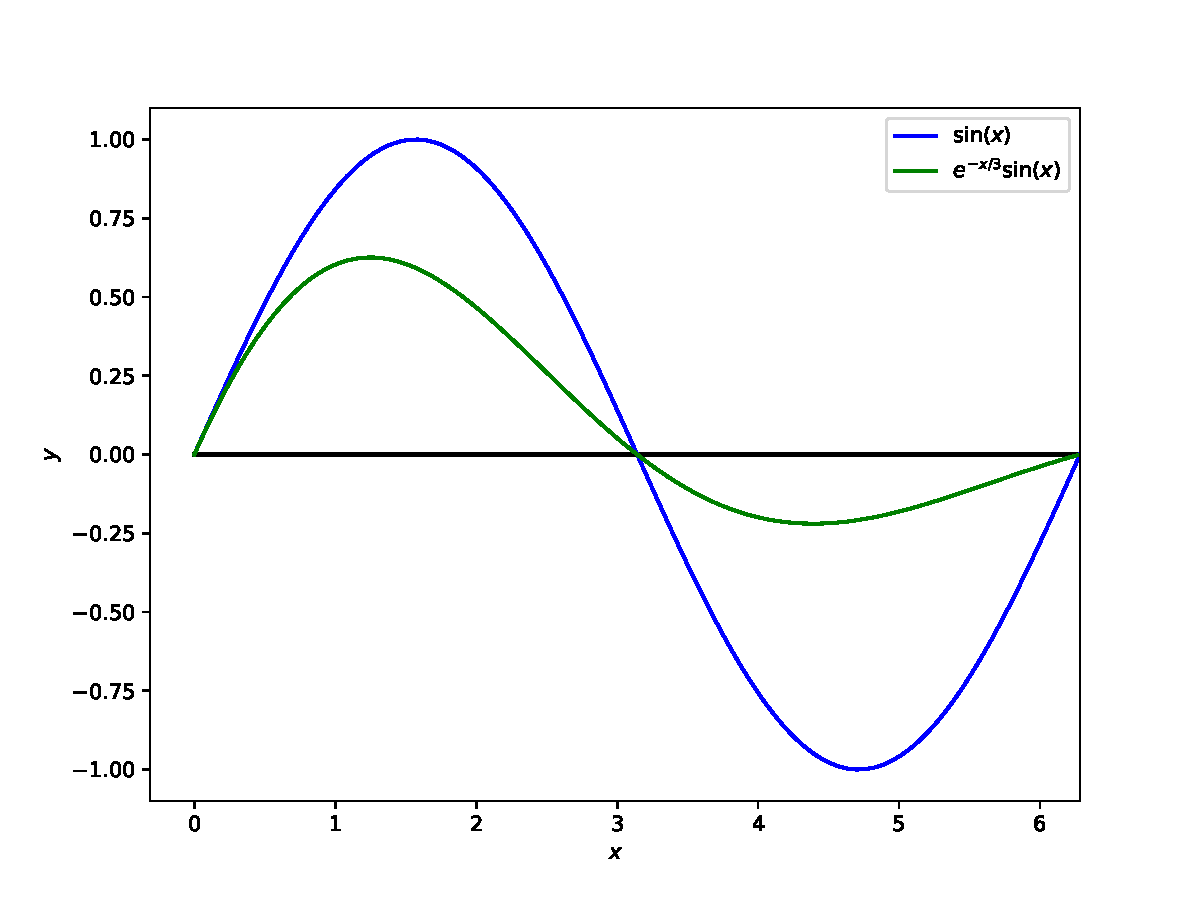
\includegraphics[width=\textwidth]{sine}%{Chapter-2/figs/sine}
\caption{This figure has been turned sideways.  With large figures, 
         the author must ensure that there are at least two double spaces
         between the caption and the page number.}
\label{fig:hist}
\end{figure}
\end{landscape}
\restoregeometry
\pagestyle{plain}
\thispagestyle{plain}
\newgeometry{margin=1in,lmargin=1.25in,footskip=\chapterfootskip, includehead, includefoot}


\section{Matrices}
Let's look at a simple example of a matrix:
\[ \left( \begin{array}{ccc}
a & b & c \\
d & e & f \\
g & h & i \end{array} \right)\] 
%
You may prefer to write it this way:
\[ \left[\begin{array} {cccccc}
1 & 0 & 0 & 0 & 0 & 0 \\
0 & 1 & 0 & 0 & 0 & 0 \\
0 & 0 & 1 & 0 & 0 & 0 \\
0 & 0 & 0 & 1 & 0 & 0 \\
0 & 0 & 0 & 0 & 1 & 0 \\
0 & 0 & 0 & 0 & 0 & 1 \\
\end{array} \right] \]

\chapter{LOREM IPSUM}

\section*{A First Section}

\paragraph{Filler Text} \lipsum[1-6]
%
\begin{figure}[t]
  \centering
  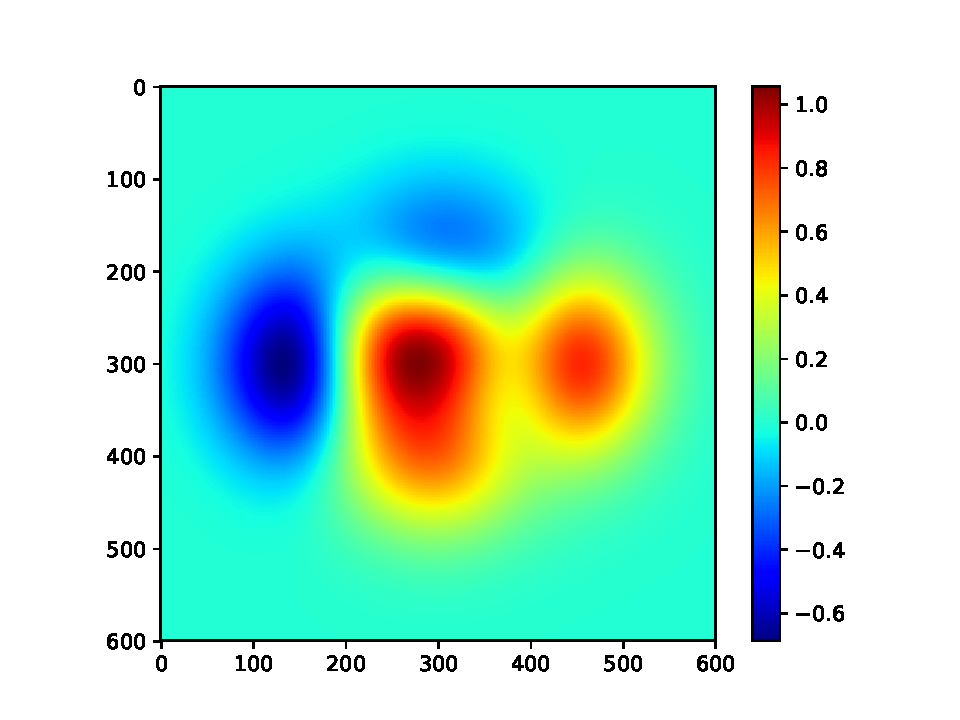
\includegraphics[width=0.6\textwidth]{color}%{Chapter-2/figs/color}
  \caption{A figure at the top of the page.}
  \label{fig:ch3.1}
\end{figure}
%
\lipsum[7-13]
%
\begin{figure}[!h]
  \centering
  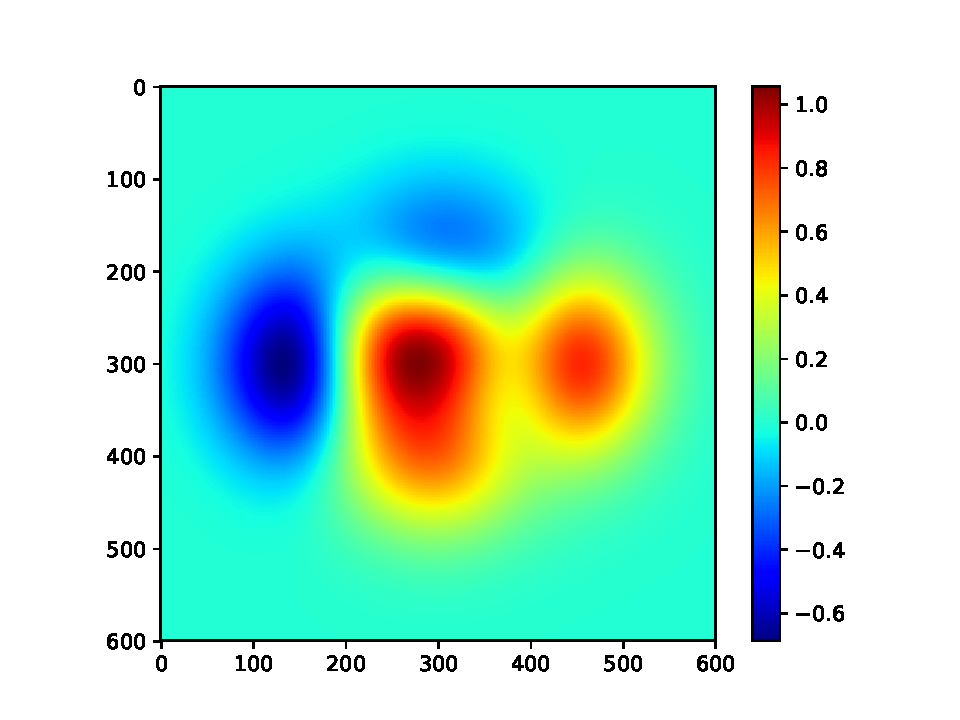
\includegraphics[width=0.6\textwidth]{color}%{Chapter-2/figs/color}
  \caption{A figure in the middle of text.}
  \label{fig:ch3.2}
\end{figure}
%
\begin{figure}[!b]
  \centering
  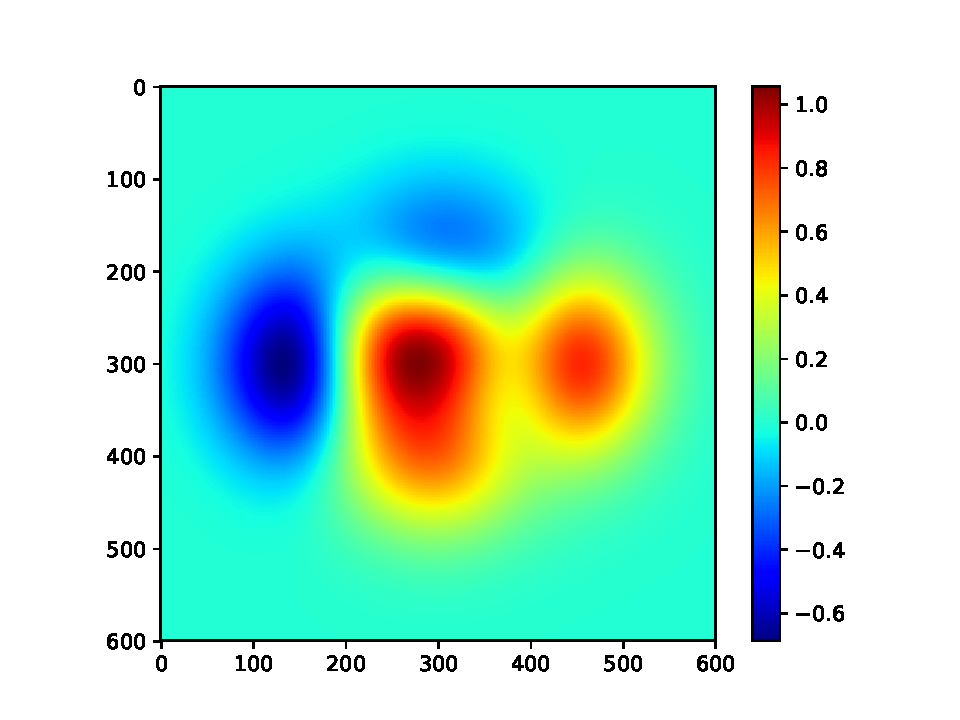
\includegraphics[width=0.6\textwidth]{color}%{Chapter-2/figs/color}
  \caption{A figure at the bottom of the page.}
  \label{fig:ch3.3}
\end{figure}
%
\lipsum[14-20]

%\include{Chapter-4/Chapter-4}
%\include{Chapter-5/Chapter-5}
%\include{Chapter-6/Chapter-6}
%\restoregeometry


%%---------------------------------------------------------------------------%%
%%  Bibliography 
%\ensureoddstart
\begin{spacing}{1}
 \setlength\bibitemsep{11pt} %22pt = 2*11pt, where fontsize is 11pt
 \phantomsection
 %\textorpdfstring and \uppercase needed due to hyperref package 
 % http://www.latex-community.org/forum/viewtopic.php?f=44&t=16601
 \addcontentsline{toc}{chapter}{\bibname}
 %\vspace{-0.5in}
\titleformat{\chapter}[display]{\bf\filcenter
}{\chaptertitlename\ \thechapter}{11pt}{\bf\filcenter}
\titlespacing*{\chapter}{0pt}{-0.5in-9pt}{22pt}

\printbibliography[heading=myheading]
\end{spacing}
%\bibliographystyle{apalike}

%%---------------------------------------------------------------------------%%
% Appendices
%\ensureoddstart
\restoregeometry
\appendix
\newgeometry{margin=1in,lmargin=1.25in,footskip=\chapterfootskip, includehead,
  includefoot}

\chapter{LOREM IPSUM}

\section{A First Section}

\paragraph{Filler Text} \lipsum[1-6]
%
\begin{figure}
  \centering
  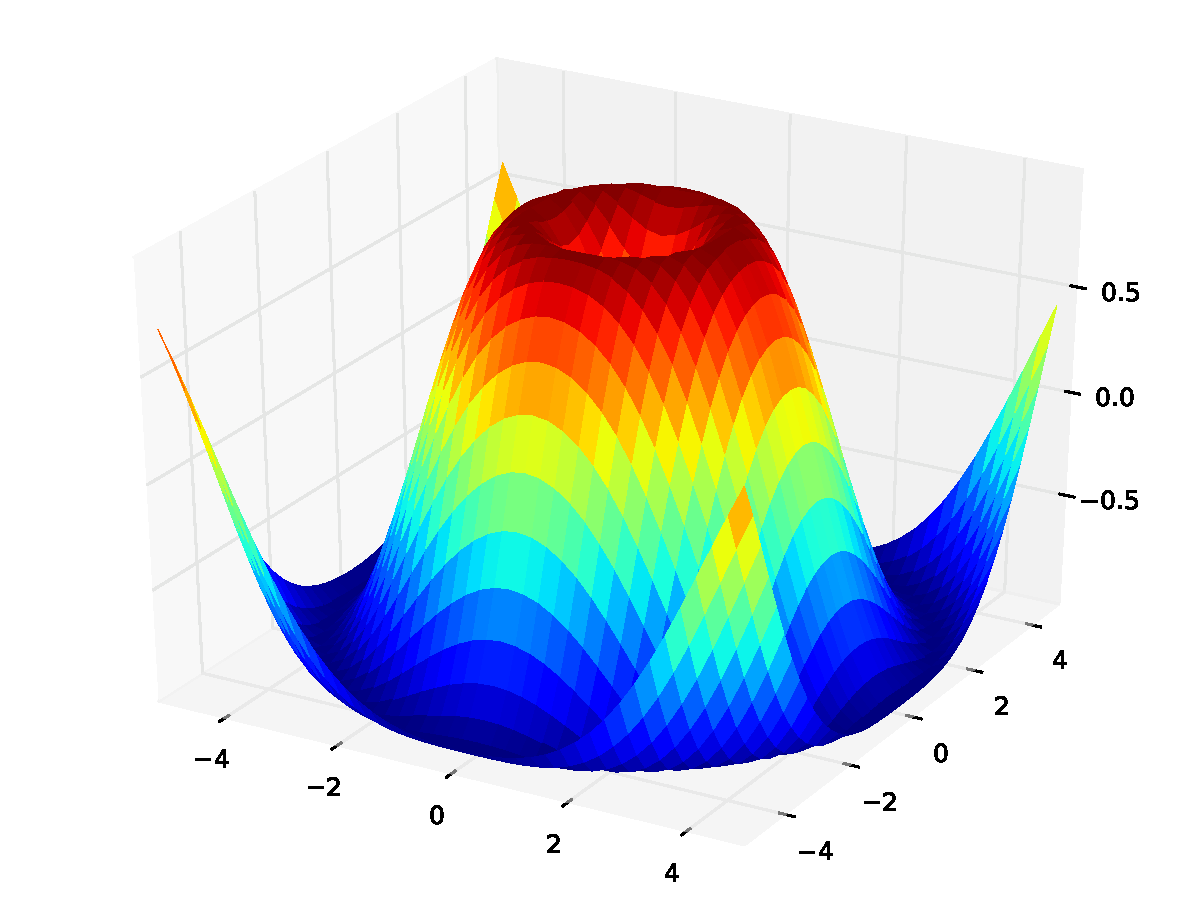
\includegraphics[width=0.6\textwidth]{Chapter-2/figs/threed}
  \caption{A figure in the appendix.}
  \label{fig:app}
\end{figure}
%
\lipsum[7-10]
\begin{table}
  \caption{A table in the appendix.}
  \label{tab:app}
  \begin{center}
    \begin{tabular}{lc}
      \toprule
      System & Author \\
      \midrule
      \TeX   & Donald Knuth   \\
      \LaTeX & Leslie Lamport \\
      \bottomrule
    \end{tabular}
  \end{center}
\end{table}
%

\section{A Second Section}

\lipsum[14-15]


\restoregeometry

%%---------------------------------------------------------------------------%%
%\ensureoddstart
\backmatter

\end{document}
